\section{NovelGridworlds}
\label{sec:novelgridworlds}

NovelGridworlds\footnote{The open-source NovelGridworlds repository is available at \url{https://github.com/gtatiya/gym-novel-gridworlds}. Additional implementation details, including environment wrappers, observation space configurations, and trajectory recording utilities, are described in~\citet{goel2021novelgridworlds}.} is an OpenAI Gym-based benchmark environment designed for developing and evaluating AI agents that can detect and adapt to novelties in open worlds. The environment provides four crafting tasks of increasing complexity, a taxonomy of twelve novelties per task, cross-platform support through a socket interface, and evaluation metrics for both planning and reinforcement learning agents.

\subsection{Environment Design}
\label{sec:ngw_environment}

Each NovelGridworlds environment is a discrete gridworld of configurable size. The arena is enclosed by unbreakable walls and contains a crafting table, an agent, free space (air blocks), and task-specific objects. At each time step, the agent selects from a discrete set of actions and maintains an inventory of collected items. The environment returns an action cost for each action taken, enabling plan-cost-based evaluation. All environments share a common set of primitive actions: \texttt{move-forward}, \texttt{turn-left}, \texttt{turn-right}, and \texttt{break}. Task-specific actions extend this set to support crafting and resource extraction.

\begin{figure}[t]
    \centering
    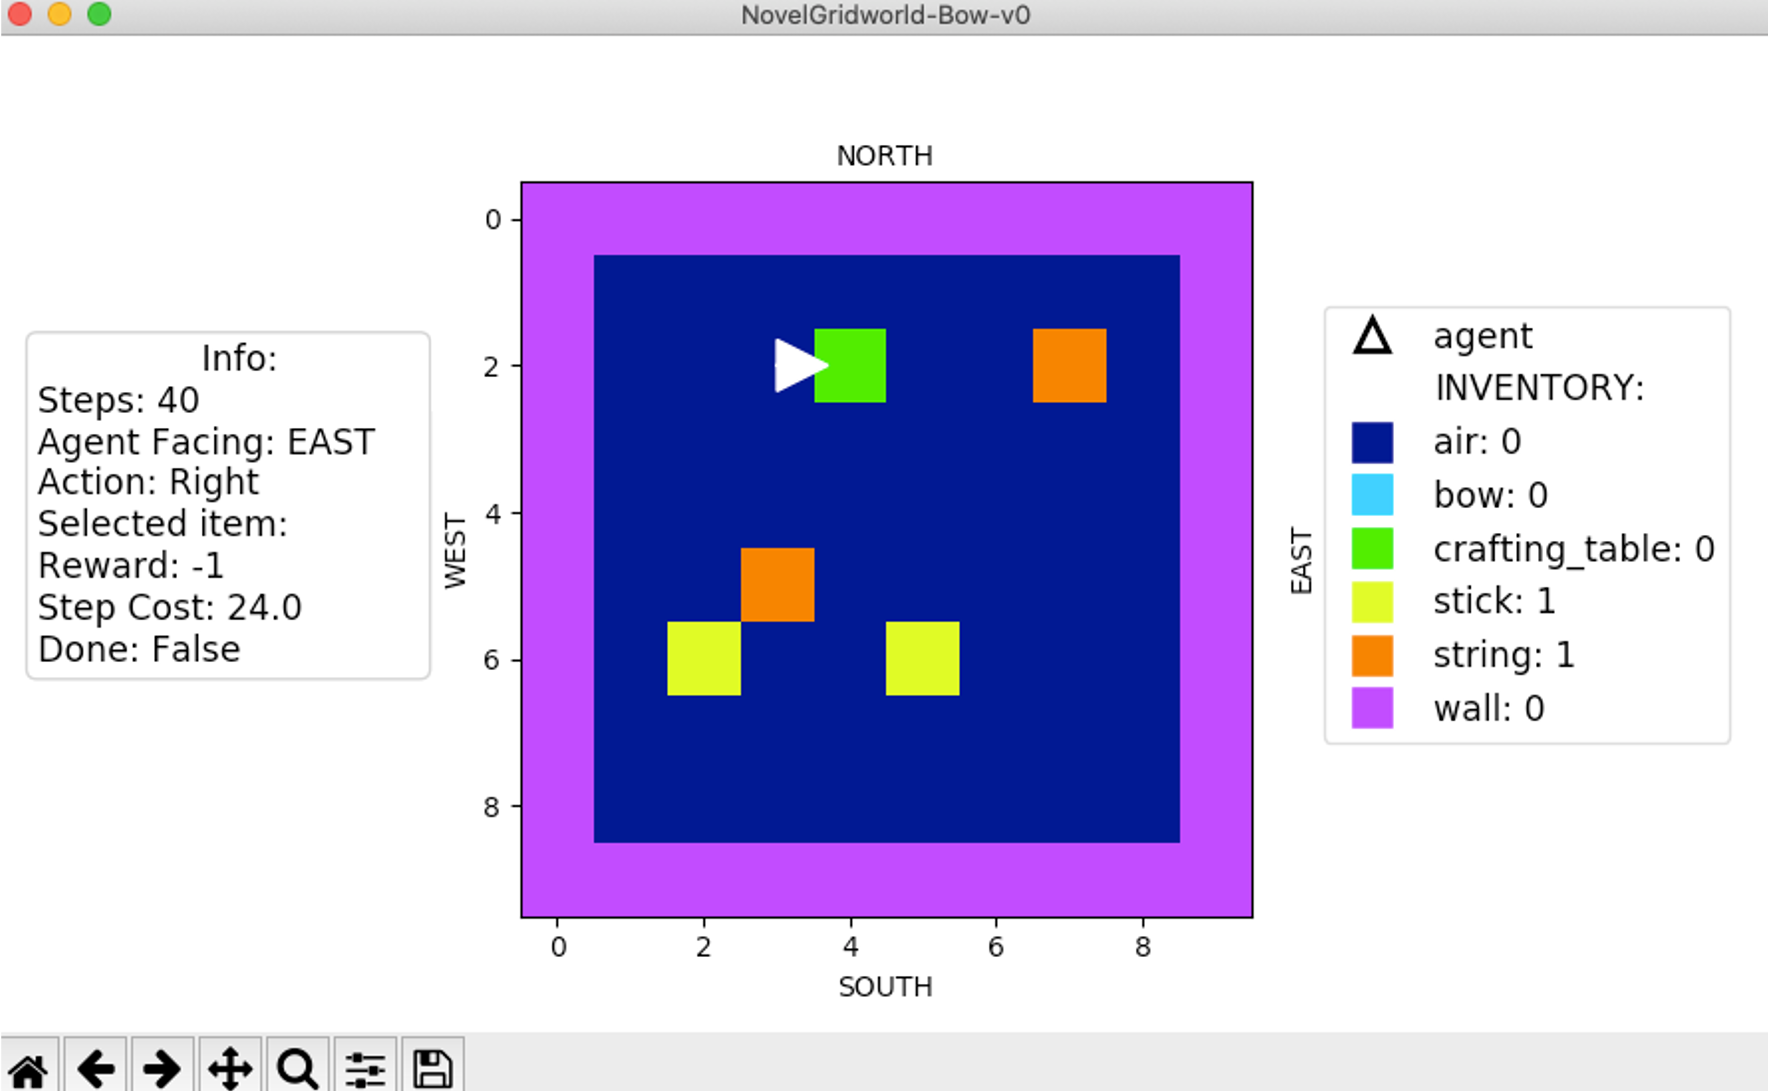
\includegraphics[width=0.8\textwidth]{figures/chapter3/screen-shot_ng.png}
    \caption{Screenshot of the NovelGridworld-Bow-v0 environment. The agent (triangle) faces the crafting table (green). Sticks (yellow) and strings (orange) are distributed in the gridworld. Blue spaces represent air blocks through which the agent can navigate, and purple blocks represent walls.}
    \label{fig:ngw_screenshot}
\end{figure}

Four tasks are implemented, each requiring the agent to craft a target item by collecting resources and applying recipes in the correct sequence:
\begin{enumerate}[leftmargin=*]
    \item \textbf{NovelGridworld-Bow-v0}: The agent collects three sticks and three strings from the environment and crafts a bow at the crafting table.
    \item \textbf{NovelGridworld-Bow-v1}: An advanced version of the previous task in which the agent must collect raw materials (tree logs and wool) and craft intermediary items (planks, sticks, and strings) before crafting the bow.
    \item \textbf{NovelGridworld-Pogostick-v0}: The agent collects sticks, planks, and rubber (extracted using a tree tap) to craft a pogostick.
    \item \textbf{NovelGridworld-Pogostick-v1}: An advanced version in which the agent must craft all intermediary items, including the tree tap itself, from raw tree logs before crafting the pogostick.
\end{enumerate}

The environment communicates with agents through a socket interface, enabling agents implemented in different programming languages to interact with the same environment. This design supports both planning agents implemented in Java-based architectures and reinforcement learning agents implemented in Python.


\subsection{Novelty Taxonomy}
\label{sec:ngw_novelty_taxonomy}

A central contribution of NovelGridworlds is a structured taxonomy for classifying novelties along two dimensions. The first dimension categorizes novelties by which component of the agent's model they affect. The second dimension characterizes the impact of the novelty on task performance.

\paragraph{Novelty classes.} Using the formalism from \cref{sec:symbolic_planning,sec:rl}, novelties are classified into three classes based on the component they alter:
\begin{itemize}[leftmargin=*]
    \item \textbf{Object novelty}: A previously unknown entity appears in the environment, altering the observation space. The resulting state $s' \in \States$ does not come from the distribution of states the agent has previously encountered.
    \item \textbf{Attribute novelty}: The properties of existing entities change, modifying the transition dynamics. Formally, the transition function changes such that for some known state-action pair $(s, a)$, the resulting state $\Transition(\cdot \mid s, a)$ differs from what the agent has previously observed.
    \item \textbf{Action novelty}: The behavior of actions changes. An action that previously produced a known effect now produces a different outcome, or new actions become available.
\end{itemize}

\paragraph{Novelty types.} Each novelty is further classified by its impact on the agent's task performance:
\begin{itemize}[leftmargin=*]
    \item \textbf{Beneficial}: The novelty helps the agent complete the task more efficiently.
    \item \textbf{Detrimental}: The novelty hinders or prevents task completion unless the agent adapts.
    \item \textbf{Irrelevant}: The novelty does not affect the task and can be safely ignored.
\end{itemize}

\begin{figure}[t]
    \centering
    \begin{subfigure}[t]{0.32\textwidth}
        \centering
        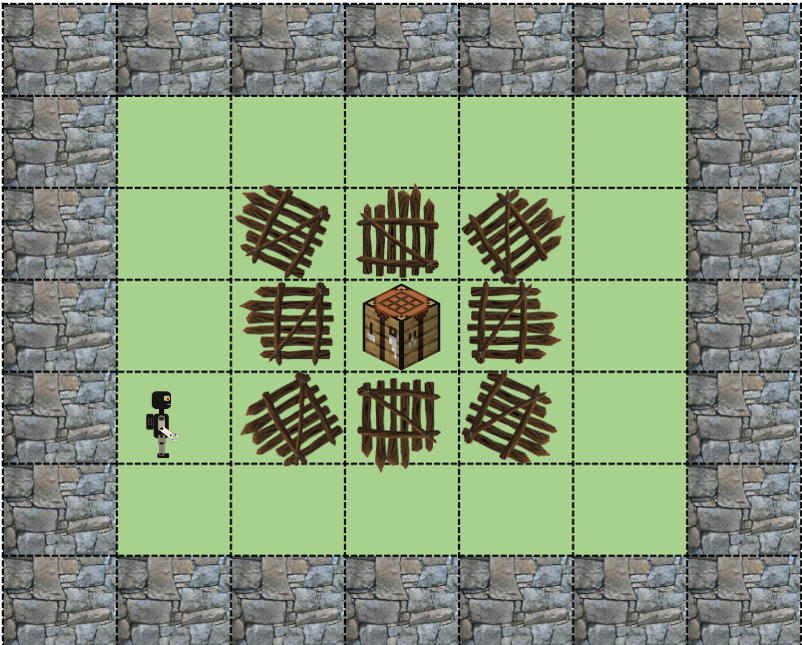
\includegraphics[width=\linewidth,keepaspectratio]{figures/chapter3/gridworld_fence.png}
        \caption{Fence (object, detrimental)}
        \label{fig:ngw_novelty_fence}
    \end{subfigure}
    \hfill
    \begin{subfigure}[t]{0.32\textwidth}
        \centering
        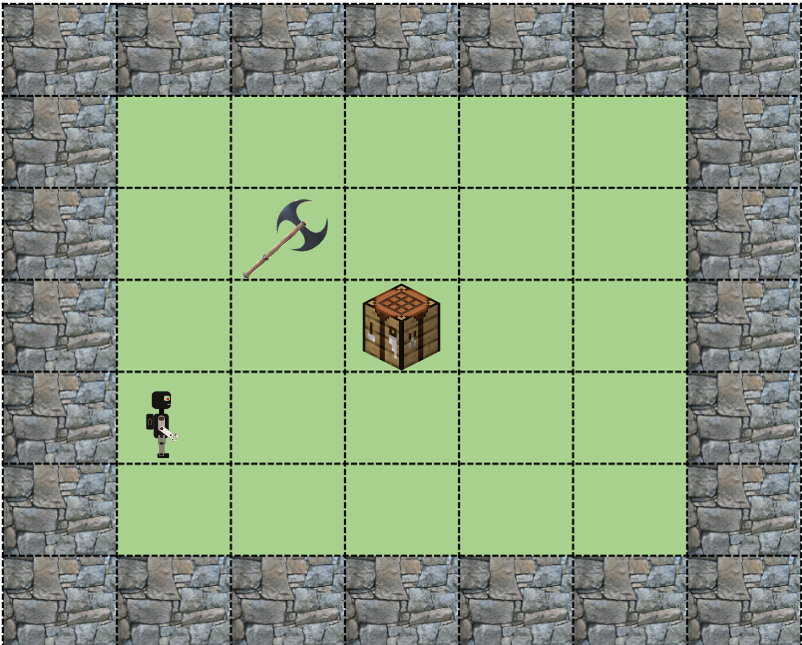
\includegraphics[width=\linewidth,keepaspectratio]{figures/chapter3/gridworld_axe.png}
        \caption{Axe (object/attribute, beneficial)}
        \label{fig:ngw_novelty_axe}
    \end{subfigure}
    \hfill
    \begin{subfigure}[t]{0.32\textwidth}
        \centering
        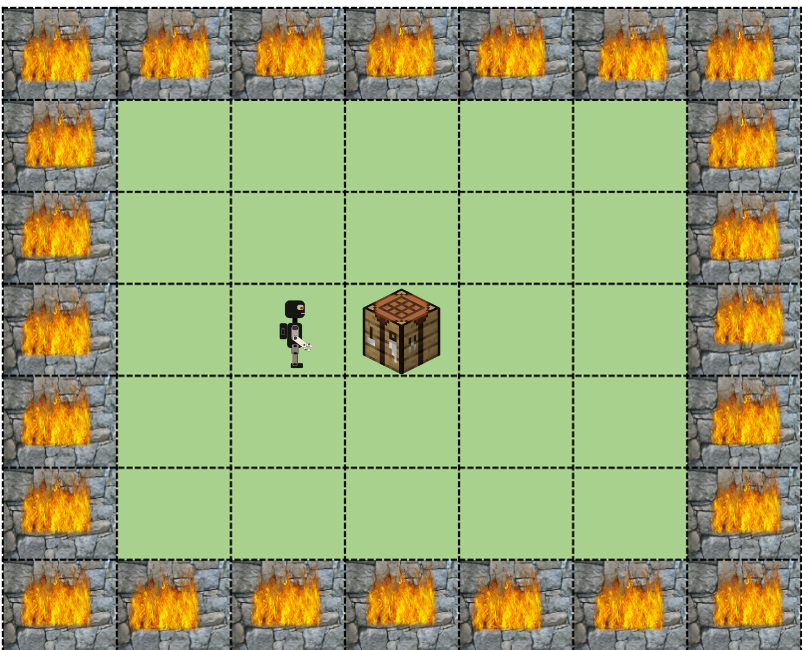
\includegraphics[width=\linewidth,keepaspectratio]{figures/chapter3/gridworld_firewall4.png}
        \caption{Fire wall (object/attribute, detrimental)}
        \label{fig:ngw_novelty_firewall}
    \end{subfigure}
    \caption{Representative NovelGridworlds novelty scenarios discussed in the evaluation (fence, axe, and fire wall). Each panel shows how the grid layout and entities change under the corresponding novelty.}
    \label{fig:ngw_novelty_examples}
\end{figure}

Twelve novelties are implemented across all four tasks, spanning all combinations of class and type. Examples include a \emph{fence} (object, detrimental) that obstructs access to resources, an \emph{axe} (object and attribute, beneficial) that doubles the yield from breaking objects, \emph{break increase} (attribute, beneficial) that provides additional items upon breaking, \emph{fire wall} (object and attribute, detrimental) that causes episode termination upon contact, and \emph{action remapping} (action, detrimental) that randomly shuffles the effects of the agent's actions. Some novelties span multiple classes; for instance, \emph{axe-to-break} introduces a new object, adds a new action, and modifies the transition dynamics of the break action, spanning all three classes simultaneously.


\subsection{Evaluation Metrics}
\label{sec:ngw_metrics}

NovelGridworlds introduces three evaluation metrics designed to capture different aspects of an agent's response to novelty:
\begin{itemize}[leftmargin=*]
    \item \textbf{Metric M1 (Reaction Performance)}: The ratio of cumulative action cost in the post-novelty scenario to the cost in the pre-novelty scenario. A ratio greater than 1 indicates degraded performance, less than 1 indicates improvement, and equal to 1 indicates no change.
    \item \textbf{Metric M2 (Steps)}: The number of steps the agent takes to complete the task in the post-novelty scenario.
    \item \textbf{Metric M3 (Detection Rate)}: A binary indicator of whether the agent correctly reports the presence of a novelty. This metric is specific to agents with explicit novelty detection mechanisms, such as planning agents.
\end{itemize}


\subsection{Experimental Results}
\label{sec:ngw_results}

Two types of agents were evaluated: a symbolic planning agent implemented using the DIARC cognitive architecture~\citep{schermerhorn2006diarc, scheutz2019diarc} with the MetricFF planner~\citep{hoffmann2003metricff}, and a reinforcement learning agent trained using Proximal Policy Optimization (PPO)~\citep{schulman2017proximal}. The RL agent used a LiDAR-like observation space consisting of eight beams at $45^\circ$ increments, each returning the Euclidean distance to the nearest object, augmented by inventory and selected-item vectors.

\begin{table}[t]
\centering
\footnotesize
\caption{Performance of the planning agent across four tasks. Each task reports pre-novelty (Default) and post-novelty (Fence, Arrow/Spring, Axe) scenarios.}
\label{tab:ngw_results}
\begin{tabular}{lcccc}
\toprule
\textbf{Metrics} & \textbf{Default} & \textbf{Fence} & \textbf{Arrow/Spring} & \textbf{Axe} \\
\midrule
\multicolumn{5}{c}{\textbf{NovelGridworld-Bow-v0}} \\
\midrule
M1 & $1.00 \pm 0.00$ & $1.80 \pm 0.15$ & $1.11 \pm 0.135$ & $1.02 \pm 0.04$ \\
M2 & $87.6 \pm 16.8$ & $123.0 \pm 18.0$ & $90.6 \pm 15.1$ & $98.0 \pm 15.9$ \\
\addlinespace
\multicolumn{5}{c}{\textbf{NovelGridworld-Bow-v1}} \\
\midrule
M1 & $1.00 \pm 0.00$ & $1.82 \pm 0.24$ & $1.00 \pm 0.02$ & $0.99 \pm 0.02$ \\
M2 & $36.8 \pm 6.5$ & $54.2 \pm 4.8$ & $37 \pm 5.4$ & $35.4 \pm 4.0$ \\
\addlinespace
\multicolumn{5}{c}{\textbf{NovelGridworld-Pogostick-v0}} \\
\midrule
M1 & $1.00 \pm 0.00$ & $1.16 \pm 0.08$ & $0.97 \pm 0.03$ & $0.99 \pm 0.04$ \\
M2 & $127.8 \pm 9.0$ & $122.0 \pm 19.8$ & $105.6 \pm 15.7$ & $114.8 \pm 4.0$ \\
\addlinespace
\multicolumn{5}{c}{\textbf{NovelGridworld-Pogostick-v1}} \\
\midrule
M1 & $1.00 \pm 0.00$ & $1.34 \pm 0.06$ & $1.07 \pm 0.05$ & $0.99 \pm 0.02$ \\
M2 & $94.2 \pm 12.9$ & $105.2 \pm 14.5$ & $100.8 \pm 22.58$ & $85.0 \pm 15.4$ \\
\bottomrule
\end{tabular}
\end{table}



\paragraph{Planning agent.} The planning agent was evaluated across all four tasks under three novelties (fence, arrow/spring, and axe); results are reported in \cref{tab:ngw_results}. The agent achieved a 100\% detection rate (M3) in all scenarios. Under the fence novelty, the cost ratio M1 consistently exceeded 1 across all tasks (for example, $1.80 \pm 0.15$ in Bow-v0 and $1.34 \pm 0.06$ in Pogostick-v1), reflecting the additional cost of breaking fences to access resources. Under irrelevant novelties (arrow/spring), the agent's performance remained close to the pre-novelty baseline, as expected. The axe novelty, although beneficial, produced negligible improvement because the agent did not always discover or exploit the new object.

\paragraph{Reinforcement learning agent.} The RL agent was evaluated on the Bow-v0 task under three novelties: action remapping, fire wall, and break increase. The agent achieved a 92\% success rate on the base task after 1.8 million training time steps. Under the beneficial break-increase novelty, cumulative reward improved but the success rate dropped to 29.2\%, suggesting the agent learned to hoard resources rather than complete the task. The fire-wall novelty caused a complete failure, with 0\% success rate, as the agent could not learn to avoid the lethal walls. Action remapping showed an average 12\% decline in success rate, though performance varied substantially across trials depending on how severely the action mapping was shuffled.

\begin{figure}[t]
    \centering
    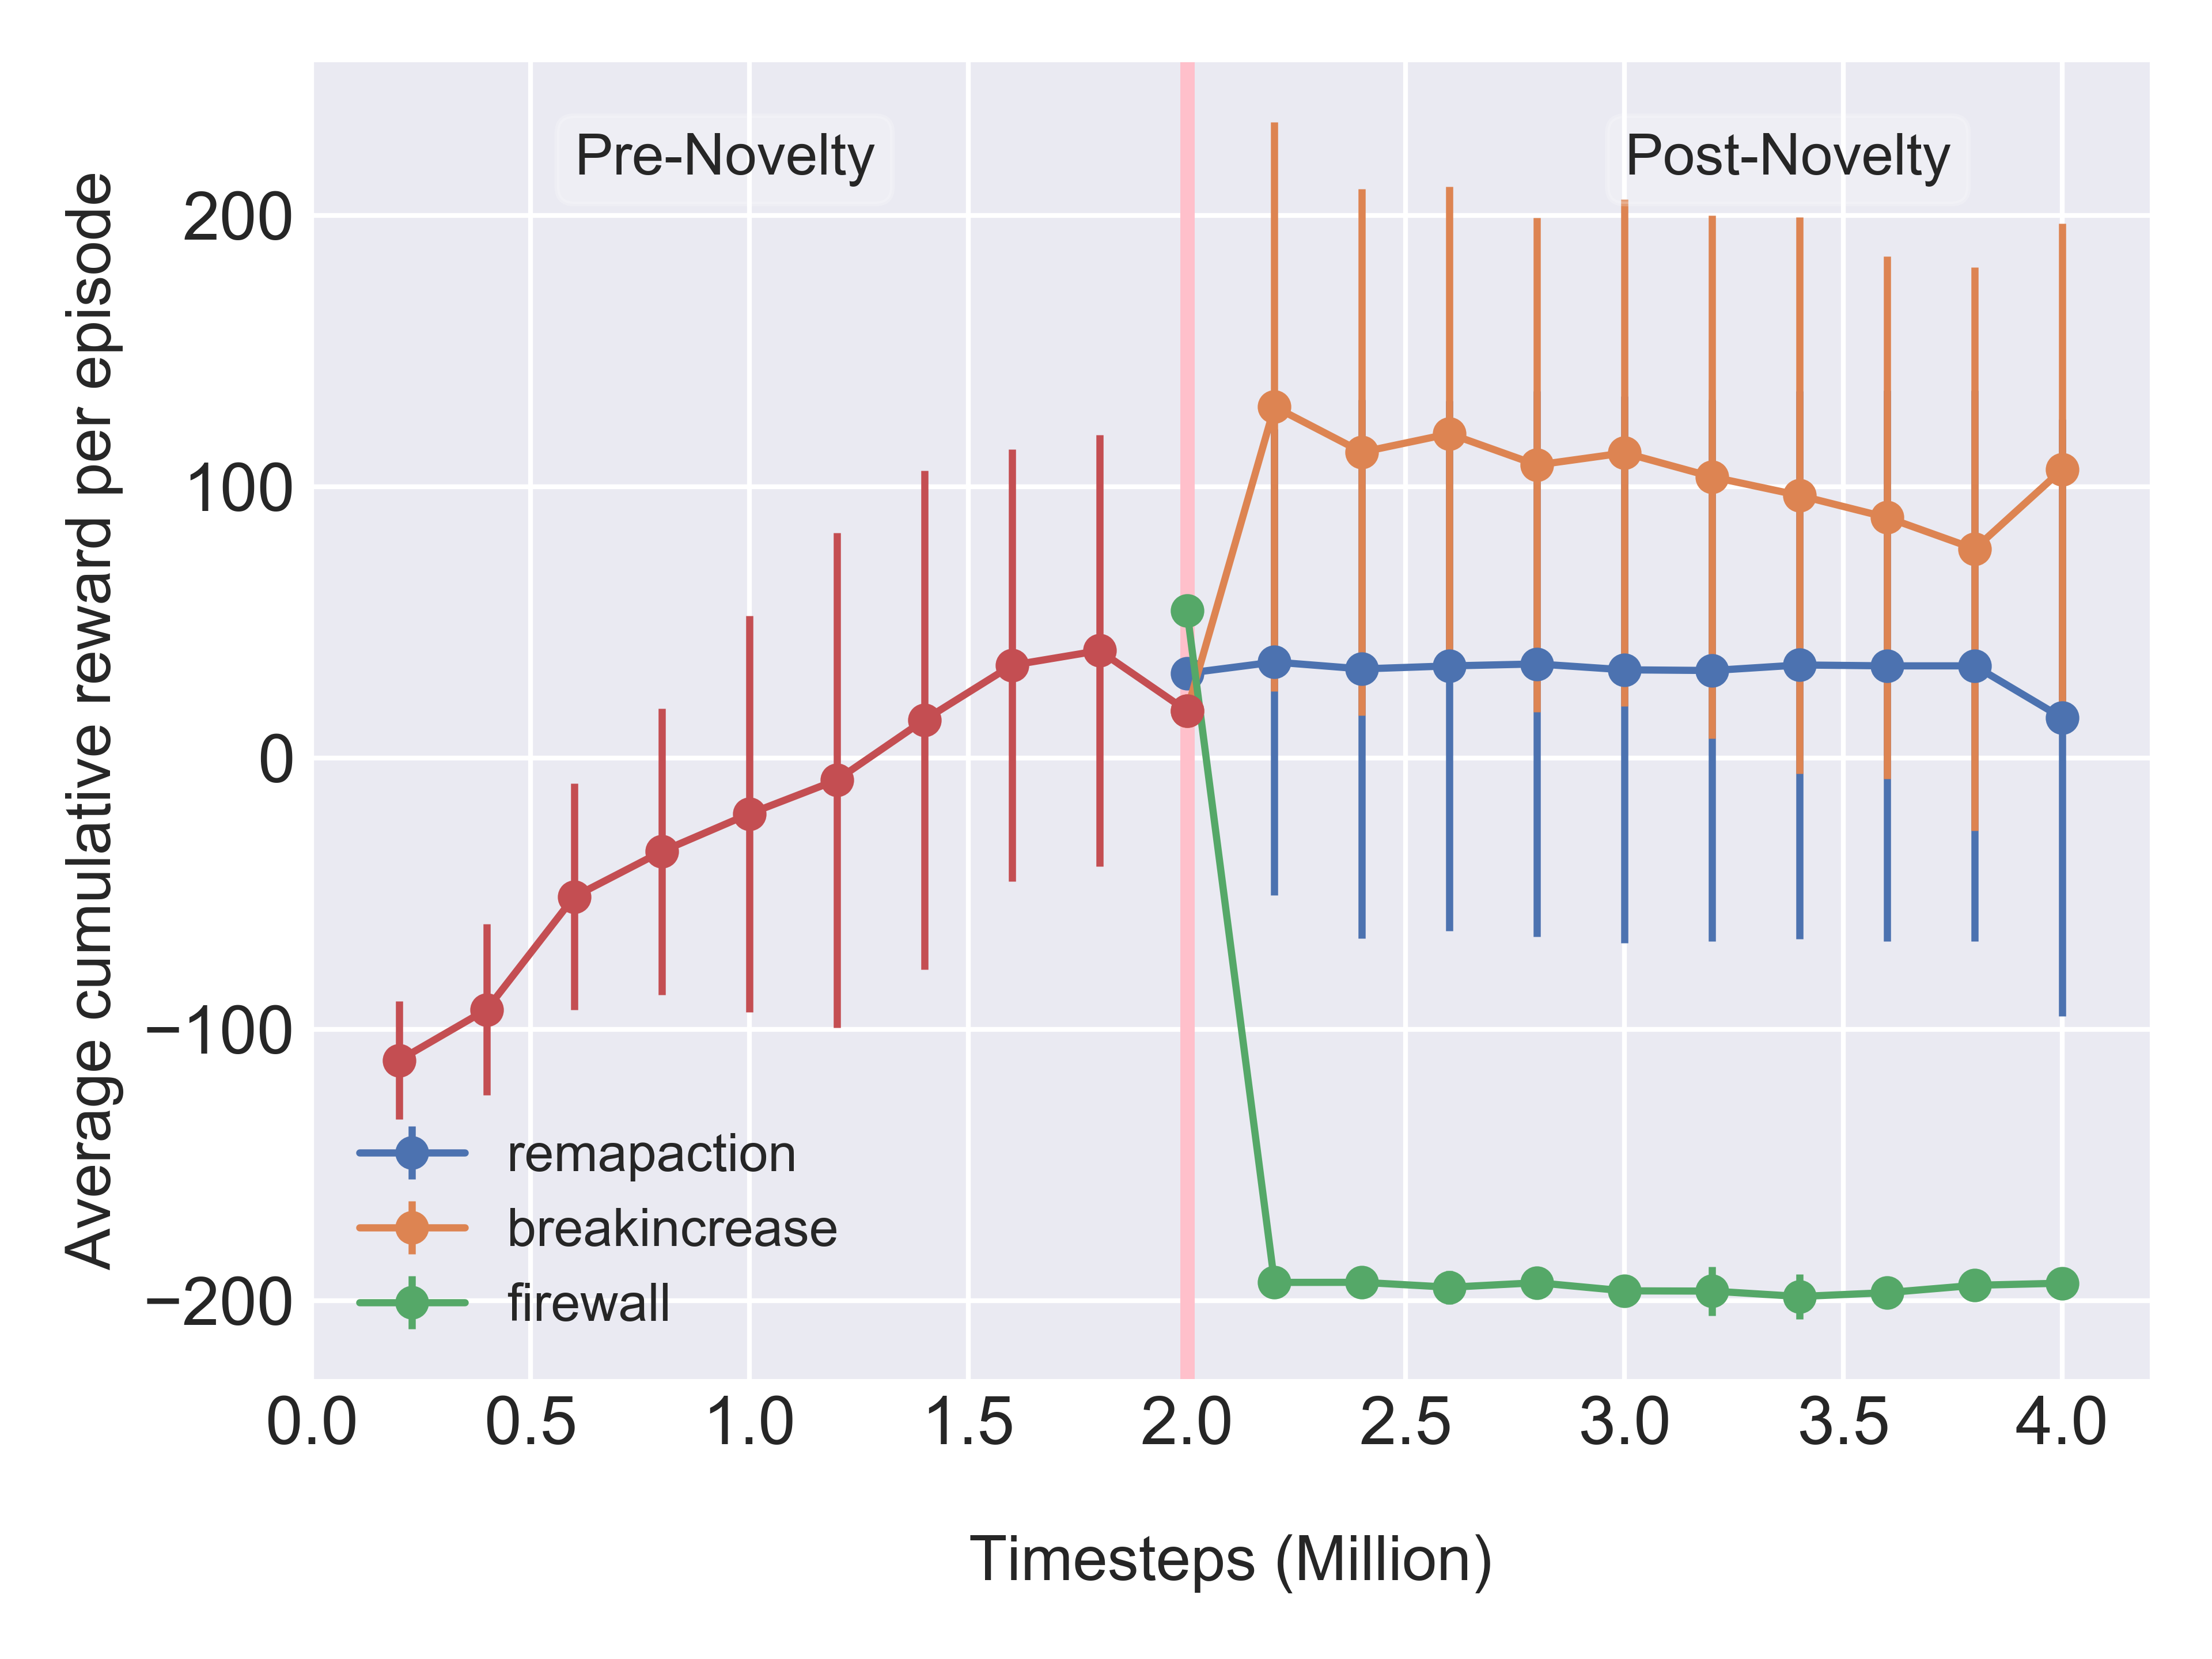
\includegraphics[width=0.8\textwidth]{figures/chapter3/results_latest.png}
    \caption{Learning performance of the RL agent on NovelGridworld-Bow-v0. The vertical line at 2 million time steps marks the introduction of novelty. Break increase (orange) shows improved reward but reduced success rate. Fire wall (green) causes complete failure. Action remapping (blue) shows partial recovery.}
    \label{fig:ngw_rl_curves}
\end{figure}


\subsection{Key Insights}
\label{sec:ngw_insights}

The NovelGridworlds experiments reveal a fundamental tension between the two dominant paradigms for sequential decision-making. Planning agents, equipped with explicit models of the environment, excel at detecting novelties through discrepancies between expected and observed states. However, they lack mechanisms for adapting their models in response to detected novelties, and their performance degrades gracefully but without recovery. Reinforcement learning agents, in contrast, can potentially adapt through continued interaction but suffer from high sample complexity and are brittle when novelties alter the observation space or introduce lethal states. Neither paradigm alone is sufficient for robust open-world operation. These observations directly motivate the development of hybrid approaches, as well as a more flexible evaluation ecosystem, which we present in the next section.